
\documentclass[dvipdfmx]{jlreq}
% FIXED: 「Cannot determine size of graphic (no BoundingBox)」エラーの修正。
% OverleafでpLaTeX/upLaTeXを使う場合、PNG画像を読み込むにはdvipdfmxドライバの指定が必須です。
% クラスオプションに書くことでgraphicx・color・hyperrefすべてに適用されます。
% ※コンパイラをLuaLaTeXにしている場合は [dvipdfmx] を削除してください。
\usepackage{graphicx, color}
\usepackage[hidelinks]{hyperref} % 目次・参照にリンクを付ける
latex\renewcommand{\topfraction}{0.9}
\renewcommand{\bottomfraction}{0.8}
\renewcommand{\textfraction}{0.07}
\renewcommand{\floatpagefraction}{0.8}
\setcounter{topnumber}{3}
\setcounter{totalnumber}{5}

\title{SHAMIKO 説明書}
\author{}
\date{\today}

\begin{document}
\maketitle

\tableofcontents
\clearpage

%==============================================================
\section{SHAMIKOの概要}
%==============================================================
SHAMIKOはSAKURA-Gと同等の機能を実現することを目標として開発された、電力解析攻撃の実験用基板である。XilinxのFPGAであるSpartan-7を搭載しており、ISEではなく最新のVivadoを用いた開発が可能である。
% 引用したい場合は \cite などで文献参照を追加してください。

図\ref{fig:block_diagram}にSHAMIKOの概略図を示す。SHAMIKOには2台のFPGAが搭載されており、1台は制御及びPCとの通信用のController FPGA、もう1台は電力解析対象の回路を実装するためのMain FPGAである。
Main FPGAのロジックの電源ラインにはシャント抵抗が挿入されており、回路が演算を行う際の消費電力が電位差となって現れる。シャント抵抗の負荷側には増幅用のアンプが接続されており、電力消費によって発生した電圧変動を増幅してそのままオシロスコープに接続することが可能である。

SHAMIKOは完全にオープンソースな基板である。KiCadのプロジェクトファイルに含まれる回路図データ、基板設計データはもちろんのこと、プロジェクト固有のライブラリも含めすべて公開されており、自由に改変可能である。
SHAMIKOをベースとして自分の研究プロジェクトのためにカスタマイズを行ったり、Main FPGA部分を自らテープアウトしたICに置き換えて電力解析を行う、といった改変も可能である。

%==============================================================
\section{システム構成}
%==============================================================
SHAMIKOの全体構成を図\ref{fig:block_diagram}に示す。SHAMIKOはPCとの通信および制御を行うControl FPGAと、電流測定対象のMain FPGAから構成される。Control FPGAとMain FPGAの間は64\,bitのデータ信号と5\,bitの制御信号で接続されている。

PCとSHAMIKOの接続にはFT2232HとFT600の2つのインタフェースがあり、UARTおよびパラレルバスによる高速通信を提供する。高速通信用のポートであるFT600はControl FPGAのみに接続されている。

Control FPGAおよびMain FPGAのそれぞれには、次の4種類の回路が接続されている。
\begin{itemize}
  \item \textbf{Configuration}：FPGAの回路の記録やデバッグインタフェースを提供する
  \item \textbf{Supervisor}：FPGAのリセットやクロック供給を行う
  \item \textbf{Header}：FPGAと外部を接続するIO回路
  \item \textbf{Peripheral}：スイッチやLEDといったインタフェースを提供する
\end{itemize}

また、第\ref{sec:power_measure}節で詳しく説明するが、電力測定対象であるMain FPGAの電源にはシャント抵抗が挿入されており、その回路で電流測定を行う。

\begin{figure}[htbp]
  \centering
  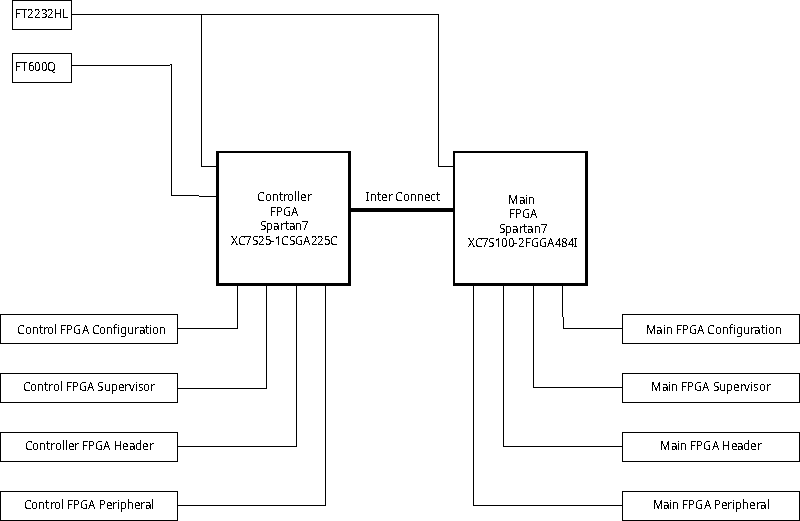
\includegraphics[width=100mm]{images/System.pdf}
  \caption{システムブロック図}
  \label{fig:block_diagram}
\end{figure}

%==============================================================
\subsection{電源システム}
\label{sec:power}
%==============================================================

\subsubsection{電源構造}
本回路の電源システムを図\ref{fig:power_tree}に示す。SHAMIKOは電流解析攻撃の実験環境であるため、通常のFPGAボードとは異なった電源構造を持っている。

まず、外部のACアダプタから入力された12\,Vの電気は、DC-DCコンバータによって1.2\,Vと5\,Vに降圧される。1.2\,V系はさらにLDOにより1.0\,Vへ降圧され、FPGAのロジック電源であるVCC\_INTとBRAMの電源であるVCC\_BRAMに供給される。1.0\,V系はControl FPGA用とMain FPGA用の独立した二系統が存在する。

DC-DCとLDOの二段で降圧する理由は次の2点である。


\begin{enumerate}
  \item DC-DCで発生したノイズを軽減するため。
  \item LDOのドロップ電圧を下げ降圧の変換効率を上げるため。
\end{enumerate}

1.2\,V系の電源はFPGAのコア電源であるVCC\_INTを作るためだけに存在する。Controller FPGAとMain FPGAがそれぞれ独立したLDOで降圧した電源を持つ理由は、Controller FPGAの電源ラインのノイズがMain FPGAの電源ラインに影響することを防ぐためである。本基板は電力解析用のFPGA基板であるため、極力Main FPGAの電源ラインにノイズが乗らないように、ノイズの少ない電源ICを使い、重要な電源は独立させるようにしている。


5\,Vはコア電源以外の電源や、周辺回路の電源をつくるために使われる。Control FPGAおよびMain FPGA用のIOの3.3\,V電源、VCC\_AUXなどの1.8\,V電源に降圧して使われる。また、その他USBインタフェースICの3.3\,V電源などもこの5\,V電源から降圧して使われる。

電力波形の増幅用オペアンプのアナログ電源は、他のデジタル電源とは異なり12\,Vから直接降圧する形で生成されている。

\begin{figure}[htbp]
  \centering
  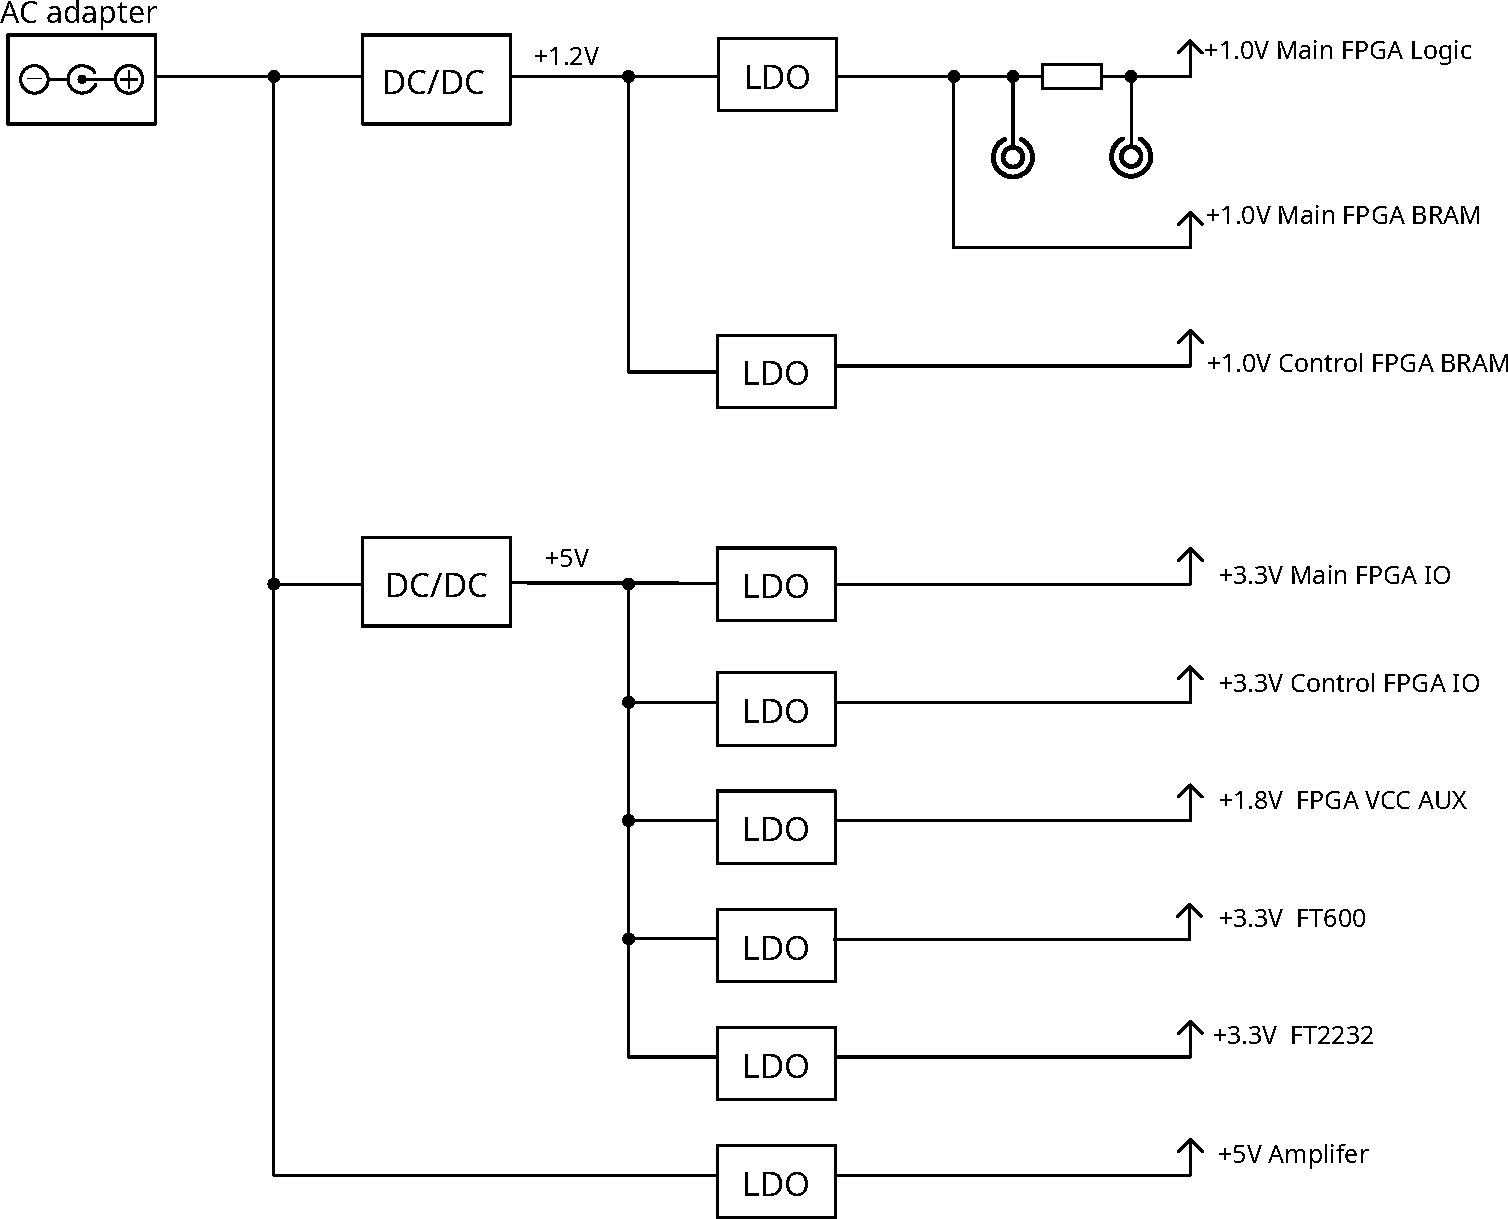
\includegraphics[width=120mm]{images/Power.pdf}
  \caption{電源系統図}
  \label{fig:power_tree}
\end{figure}

\subsubsection{電源シーケンス}
図\ref{fig:power_seq}にSHAMIKOの起動時の電源シーケンスの概略図を示す。
先にも述べた通り1.0\,Vと、1.8\,V及び3.3\,Vはそれぞれ異なるDC-DCコンバータの出力を降圧して作られる。
FPGAの電源はVCC\_INTなどのコア電圧、VCC\_AUXなどの周辺回路の電圧、IO電圧の順に一定の間隔を持って立ち上がらなければならない。
まず、1.0\,Vの電源の立ち上がりを電源シーケンスの始点とする。

1.0\,V系の電源が持つPower Goodが立ち上がってから5\,V系のDC-DCのPower Goodが立ち上がるまではおよそ8\,msであるため、5\,VのDC-DCのPGoodは1.8\,VのLDOのEN端子に接続されており、1.8\,Vは8\,ms以上遅れて立ち上がる。
1.8\,VのLDOの出力は3.3\,VのDC-DCのEN端子に接続されており、LDOの遅延機能により更に14.1\,ms遅延してからPGを出力するため、3.3\,V系が立ち上がるのは電源シーケンス開始から22\,ms後となる。これらのタイミングシーケンスはFPGAの要求するタイミング条件を満たしている。
\begin{figure}[hbtp]
  \centering
  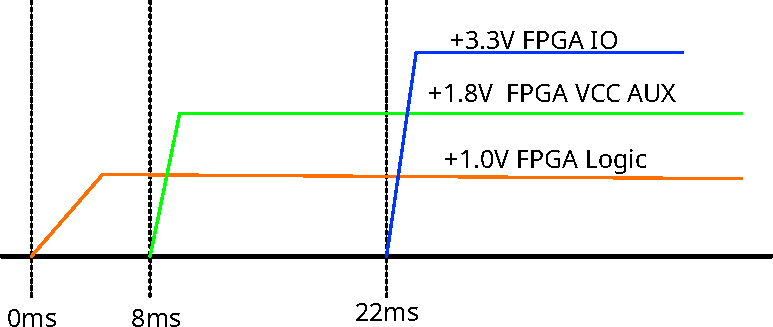
\includegraphics[width=85mm]{images/PowerSeq.pdf}
  \caption{SHAMIKOの電源シーケンス}
  \label{fig:power_seq}
\end{figure}

\subsubsection{電圧調整}
最もACアダプタに近いDC-DCコンバータはLT8625SPJV-1であり、これらの出力は1.2\,Vと5\,Vである。LT8625の出力電圧の制御はPGFB (Power Good Feedback) ピンに印加される電圧により行われ、出力電圧は
\begin{equation}
  V_{\mathrm{OUT}} = 0.5\,\mathrm{V}\,(\pm 7.5\,\%) \times \left(1 + \frac{R_{\mathrm{pull\_up}}}{R_{\mathrm{pull\_down}}}\right)
\end{equation}
の分圧比によって決定される。本システムにおけるこれらの値はデータシートのリファレンス値に基づいている。

FPGAのVCC\_INTに接続される1.0\,V系の電圧は、図\ref{fig:lt3071}に示すLT3071のV00--V02ピンのプルアップ・プルダウンにより設定される。今回の回路では1.0\,Vが所望の出力電圧であるため、V02 = Z、V01 = Z、V00 = Zに設定している。また、LT3071にはMARGという電圧の微調整を行うピンがあり、$\pm 10\,\%$の電圧調整を行うことが可能である。この端子には可変抵抗が接続されているため、電圧を変更したい際には、適宜、可変抵抗を変えて出力電圧を調整されたい。

\begin{figure}[h]
  \centering
  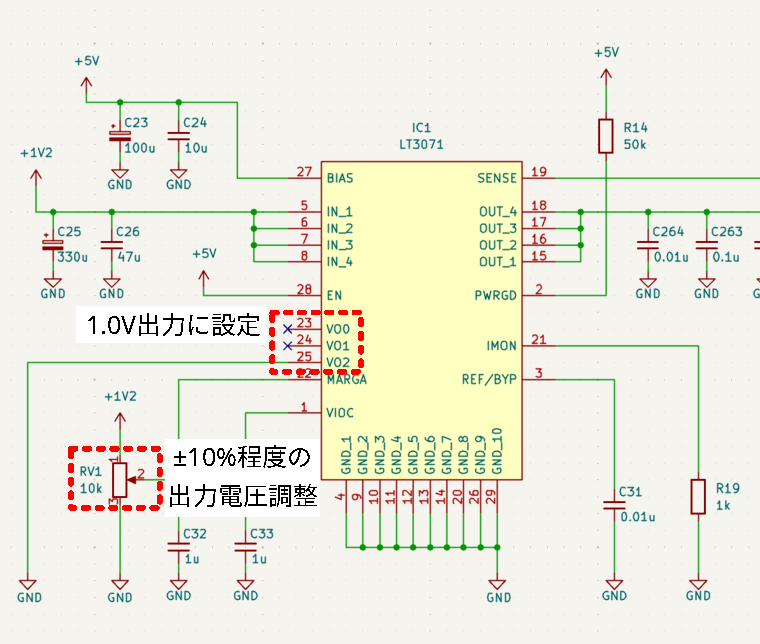
\includegraphics[width=120mm]{images/LT3071.pdf}
  \caption{LT3071による1.0\,V電源の電圧設定回路}
  \label{fig:lt3071}
\end{figure}

%==============================================================
\subsection{クロックシステム}
%==============================================================
SHAMIKOのクロック源は基板上に設置された発振子と、外部入力用のBNC端子の二種類である。図\ref{fig:clock}にそれぞれのFPGAのクロック回路の概略図を示す。
水晶発振子はシングルエンドになっており、FPGAのクロック入力端子のP側に接続されている。オシレータの型番はHCI 1532P-48.000KWVDTであり、信号周波数は48\,MHzである。BNC端子は差動ペアになっており、ファンクションジェネレータなどからクロックを入力することができる。また、GPIOピンのうち2ピンがクロックピンとして利用可能である。

\begin{figure}[htbp]
 \centering
  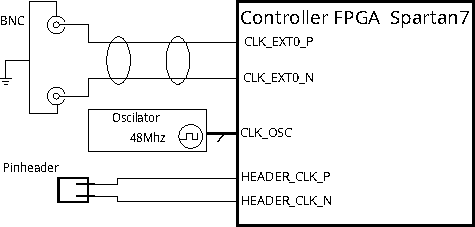
\includegraphics[width=120mm]{images/Clock.pdf}
  \caption{クロック源とFPGAとの接続}
  \label{fig:clock}
\end{figure}


Controller FPGAとMain FPGAのそれぞれのピンはそれぞれ表\ref{tb:mainclk}と表\ref{tb:ctrlclk}に示されている。

\begin{table}[htbp]
  \centering
  \begin{minipage}[t]{0.48\textwidth}
    \centering
    \caption{Main FPGAのクロックピン}
    \label{tb:mainclk}
    \begin{tabular}{|l|l|} \hline
      信号名 & Main FPGA \\ \hline \hline
      M\_CLK\_OSC & M8 \\
      M\_CLK\_EXT0\_P & T3 \\
      M\_CLK\_EXT0\_N & T2 \\
      M\_HEADER\_CLK\_P & U18 \\
      M\_HEADER\_CLK\_N & U19 \\ \hline
    \end{tabular}
  \end{minipage}\hfill
  \begin{minipage}[t]{0.48\textwidth}
    \centering
    \caption{Controller FPGAのクロックピン}
    \label{tb:ctrlclk}
    \begin{tabular}{|l|l|} \hline
      信号名 & Control FPGA \\ \hline \hline
      C\_CLK\_OSC & M9 \\
      C\_CLK\_EXT0\_P & R13 \\
      C\_CLK\_EXT0\_N & R14 \\
      C\_HEADER\_CLK\_P & H1 \\
      C\_HEADER\_CLK\_N & G1 \\ \hline
    \end{tabular}
  \end{minipage}
\end{table}

%==============================================================
\subsection{コンフィグレーション}
%==============================================================
コンフィグレーション回路の構造はControlおよびMainの両方で共通している。図\ref{fig:config}に回路図を示す。

最上段のINIT\_B、PROGRAM\_B、DONEはそれぞれコンフィグレーションのステータスを表すピンであり、LEDに接続されている。
\begin{itemize}
  \item \textbf{PROGRAM\_B}：FPGAのリセットピンのような役割であり、0\,VにすることでFPGAのすべてのコンフィグをリセットすることができる
  \item \textbf{INIT\_B}：双方向の初期化ピンであり、PROGRAM\_BがLowにされてコンフィグレーションが開始した時点でLowが出力される。このピンも同様にプルアップされている
  \item \textbf{DONE}：コンフィグレーションが完了したことを示すピン
\end{itemize}

上から2段目はコンフィグレーションモードの設定ピンであり、3\,bitある。今回の基板ではQSPIのPROMが接続されているため、PROMに書き込むためのマスターSPI（3'b001）と、デバッグに用いるJTAG（3'b101）の2つのモードを使用する。SPIのデータ信号の本数などの詳細な設定はVivadoおよびVitis上で行う。

上から3段目はJTAGピンである。今回のシステムはIOが3.3\,Vであるため、3.3\,Vの信号を入力する必要がある。JTAGコネクタとJTAGピンの間にはバッファが設置されている。

PROMはFPGAの回路構成データを格納しているROMである。SHAMIKOにはControl FPGAとMain FPGAの両方において64\,MBの容量のPROMが搭載されている。Spartan-7とPROMの間はQSPIで接続されており、Vivado上の設定から利用することができる。

\begin{figure}[htbp]
  \centering
  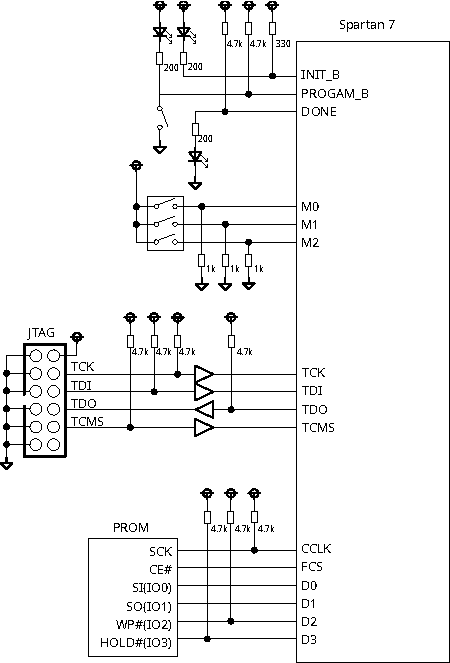
\includegraphics[width=120mm]{images/config.pdf}
  \caption{コンフィグレーション回路}
  \label{fig:config}
\end{figure}

コンフィグレーション関連信号のピン接続を表\ref{tab:config_main}および表\ref{tab:config_control}に示す。

\begin{table}[htbp]
  \centering
  \begin{minipage}[t]{0.48\textwidth}
    \centering
    \caption{Main FPGAのコンフィグレーション関連IO接続}
    \label{tab:config_main}
    \begin{tabular}{|l|l|} \hline
       信号名 &  Main FPGA \\ \hline \hline
      C\_DONE & G5  \\
      C\_INIT\_B & L5  \\
      C\_CONFIG\_M0 & M5  \\
      C\_CONFIG\_M1 & N5  \\
      C\_CONFIG\_M2 & M6  \\
      PROGRAM\_B\_0 & J5  \\
      TCK\_0 & E5  \\
      TDI\_0 & E5  \\
      TDO\_0 & K4  \\
      TMS\_0 & K5  \\
      C\_S\_CLOCK & F5  \\
      C\_S\_SELECTn & L11  \\
      C\_S\_D0 & H14  \\
      C\_S\_D1 & H15  \\
      C\_S\_D2 & J12  \\
      C\_S\_D3 & K13  \\ \hline
    \end{tabular}
    % TODO: 原文ではC_S_D0が4行重複していたためD0-D3に修正。TCK_0とTDI_0が同じE5になっている点も要確認
  \end{minipage}\hfill
  \begin{minipage}[t]{0.48\textwidth}
    \centering
    \caption{Control FPGAのコンフィグレーション関連IO接続}
    \label{tab:config_control}
    \begin{tabular}{|l|l|} \hline
       信号名 &  Control FPGA \\ \hline \hline
      M\_DONE & U4  \\
      M\_INIT\_B & Y4  \\
      M\_CONFIG\_M0 & T11  \\
      M\_CONFIG\_M1 & T10  \\
      M\_CONFIG\_M2 & U10  \\
      M\_PROGRAM\_B\_0 & U11  \\
      MX\_TCK\_0 & G9  \\
      MX\_TDI\_0 & W9  \\
      MX\_TDO\_0 & W10  \\
      MX\_TMS\_0 & Y10 \\
      M\_S\_CLOCK & D9  \\
      M\_S\_SELECTn & N17  \\
      M\_S\_D0 & M21  \\
      M\_S\_D1 & M22  \\
      M\_S\_D2 & N21  \\
      M\_S\_D3 & N22  \\ \hline
    \end{tabular}
    % TODO: 原文ではM_S_D0が4行重複していたためD0-D3に修正
  \end{minipage}
\end{table}

%==============================================================
\subsection{リセット回路}
%==============================================================
それぞれのFPGAにはリセットICが接続されており、電圧レベルが一定以上になった場合に解放されるようになっている。このうちControl FPGAのリセット回路は、USBインタフェースのリセットピンを駆動するようになっている。

%==============================================================
\subsection{インタフェース}
%==============================================================

\subsubsection{FPGA間のIO接続}
表\ref{tab:interconnect1}および表\ref{tab:interconnect2}にFPGA間の接続について示す。FPGAは64\,bitのデータ信号、2\,bitのクロック信号、4\,bitの制御信号の計70本の信号線で接続されている。それぞれの信号線の役割は固定ではないため、ユーザーは任意の機能をアサインできる。
% TODO: 本文では「5bitの制御信号」（システム構成節）と「4bitの制御信号＋2bitクロック」（本節）の記述が
% 混在しており、表にはCTRL0-CTRL4の5本が記載されています。信号の内訳を統一してください。

\begin{table}[htbp]
  \centering
  \small
  \renewcommand{\arraystretch}{0.9}
  \begin{minipage}[t]{0.48\textwidth}
    \centering
    \caption{FPGA間のIO接続（1/2）}
    \label{tab:interconnect1}
    \begin{tabular}{|l|l|l|} \hline
       信号名 & Control FPGA & Main FPGA \\ \hline \hline
    MC\_IC\_D0 & A5 & B10 \\
    MC\_IC\_D1 & A6 & A10 \\
    MC\_IC\_D2 & B6 & B9 \\
    MC\_IC\_D3 & A7 & A9 \\
    MC\_IC\_D4 & A8 & C8 \\
    MC\_IC\_D5 & A9 & B8 \\
    MC\_IC\_D6 & B9 & A7 \\
    MC\_IC\_D7 & A10 & B7 \\
    MC\_IC\_D8 & B10 & B6 \\
    MC\_IC\_D9 & A11 & A10 \\
    MC\_IC\_D10 & B11 & A5 \\
    MC\_IC\_D11 & A12 & C5 \\
    MC\_IC\_D12 & B12 & A4 \\
    MC\_IC\_D13 & A13 & B3 \\
    MC\_IC\_D14 & B13 & A3 \\
    MC\_IC\_D15 & A14 & A2 \\
    MC\_IC\_D16 & B13 & B2 \\
    MC\_IC\_D17 & B15 & B10 \\
    MC\_IC\_D18 & C14 & C2 \\
    MC\_IC\_D19 & C15 & C1 \\
    MC\_IC\_D20 & D15 & D2 \\
    MC\_IC\_D21 & E14 & D1 \\
    MC\_IC\_D22 & E15 & E12 \\
    MC\_IC\_D23 & F14 & E1 \\
    MC\_IC\_D24 & F15 & F1 \\
    MC\_IC\_D25 & G14 & G2 \\
    MC\_IC\_D26 & G15 & G1 \\
    MC\_IC\_D27 & J15 & H2 \\
    MC\_IC\_D28 & K14 & J2 \\
    MC\_IC\_D29 & K15 & J1 \\
    MC\_IC\_D30 & L14 & K2 \\ \hline
    \end{tabular}
    % TODO: D9のMain側A10がD1と重複、D17のMain側B10がD0と重複、
    % Control側B13がD14/D16で重複しています。要確認
  \end{minipage}\hfill
  \begin{minipage}[t]{0.48\textwidth}
    \centering
    \caption{FPGA間のIO接続（2/2）}
    \label{tab:interconnect2}
    \begin{tabular}{|l|l|l|} \hline
       信号名 & Control FPGA & Main FPGA \\ \hline \hline
    MC\_IC\_D31 & L15 & K1 \\
    MC\_IC\_D32 & M14 & L1 \\
    MC\_IC\_D33 & M15 & M2 \\
    MC\_IC\_D34 & N14 & M1 \\
    MC\_IC\_D35 & N15 & N1 \\
    MC\_IC\_D36 & P15 & P2 \\
    MC\_IC\_D37 & P14 & P1 \\
    MC\_IC\_D38 & C6 & D8 \\
    MC\_IC\_D39 & D7 & D7 \\
    MC\_IC\_D40 & C7 & D6 \\
    MC\_IC\_D41 & D8 & C6 \\
    MC\_IC\_D42 & C8 & D5 \\
    MC\_IC\_D43 & D9 & D4 \\
    MC\_IC\_D44 & C9 & C4 \\
    MC\_IC\_D45 & D10 & C3 \\
    MC\_IC\_D46 & C10 & E4 \\
    MC\_IC\_D47 & D11 & E3 \\
    MC\_IC\_D48 & D12 & F4 \\
    MC\_IC\_D49 & D13 & G4 \\
    MC\_IC\_D50 & E12 & G3 \\
    MC\_IC\_D51 & E13 & H4 \\
    MC\_IC\_D52 & G12 & H3 \\
    MC\_IC\_D53 & G13 & J3 \\
    MC\_IC\_D54 & H12 & K4 \\
    MC\_IC\_D55 & H13 & K3 \\
    MC\_IC\_D56 & K12 & L4 \\
    MC\_IC\_D57 & L12 & T7 \\
    MC\_IC\_D58 & L13 & M3 \\
    MC\_IC\_D59 & M13 & N4 \\
    MC\_IC\_D60 & N12 & N3 \\
    MC\_IC\_D61 & N13 & P3 \\
    MC\_IC\_D62 & N11 & R4 \\
    MC\_IC\_D63 & N10 & R3 \\
    MC\_IC\_CTRL0 & C13 & V1 \\
    MC\_IC\_CTRL1 & E11 & W1 \\
    MC\_IC\_CTRL2 & F11 & W4 \\
    MC\_IC\_CTRL3 & G11 & E5 \\
    MC\_IC\_CTRL4 & H11 & T6 \\ \hline
    \end{tabular}
  \end{minipage}
\end{table}

\newpage
\subsubsection{ FPGAのペリフェラル}
図\ref{fig:peripheral}に示すように、FPGAにはLED、タクトスイッチ、スライドスイッチが接続されている。これらはユーザー用のIOとして接続されているため、自らのアプリケーションに合わせて自由に利用することができる。詳細は回路図を参照すること。
\begin{figure}[h]
  \centering
  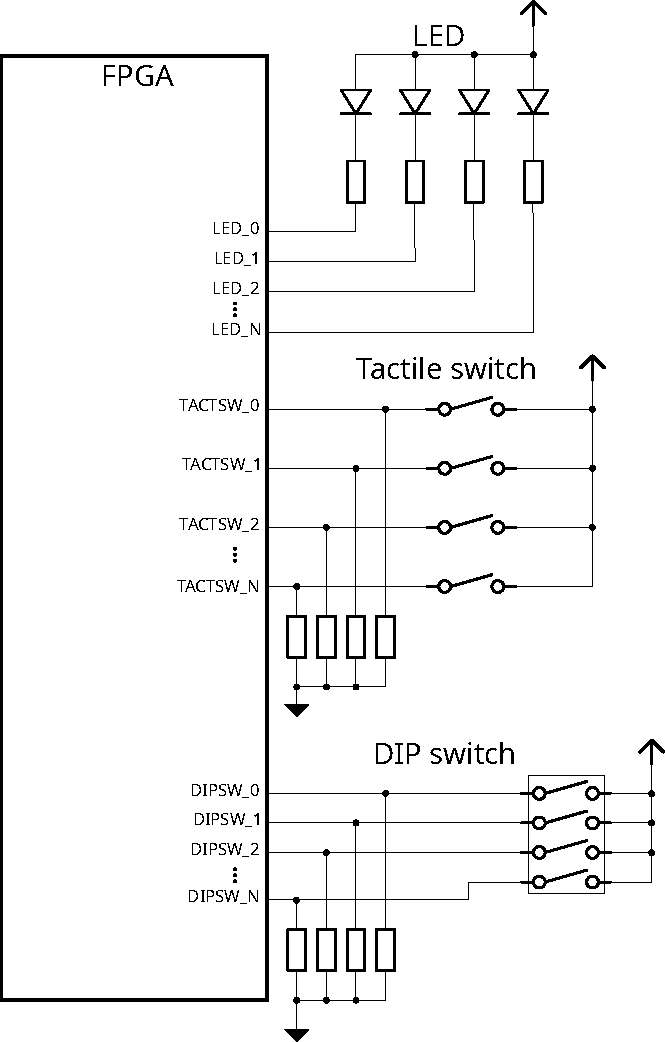
\includegraphics[width=120mm]{images/Peripheral.pdf}
  \caption{FPGAに接続された周辺回路の概略図}
  \label{fig:peripheral}
\end{figure}


図\ref{fig:pinmap_fpga}にそれぞれFPGAと汎用GPIOポートのピン配置を示す。
Controller FPGAは8本のGPIOピン、Main FPGAは26本のGPIOピンを持つ。すべてのIOポートの電圧レベルは3.3\,Vである。
これらのGPIOのうち2本はそれぞれクロック入力用のピンにアサインされている。しかしながら、これらのピンはインピーダンスの整合が取れているわけではないため、GPIOとして入力する場合でも、クロック入力として利用する場合であっても、シングルエンド入力として利用することを推奨する。

\begin{figure}[h]
  \centering
  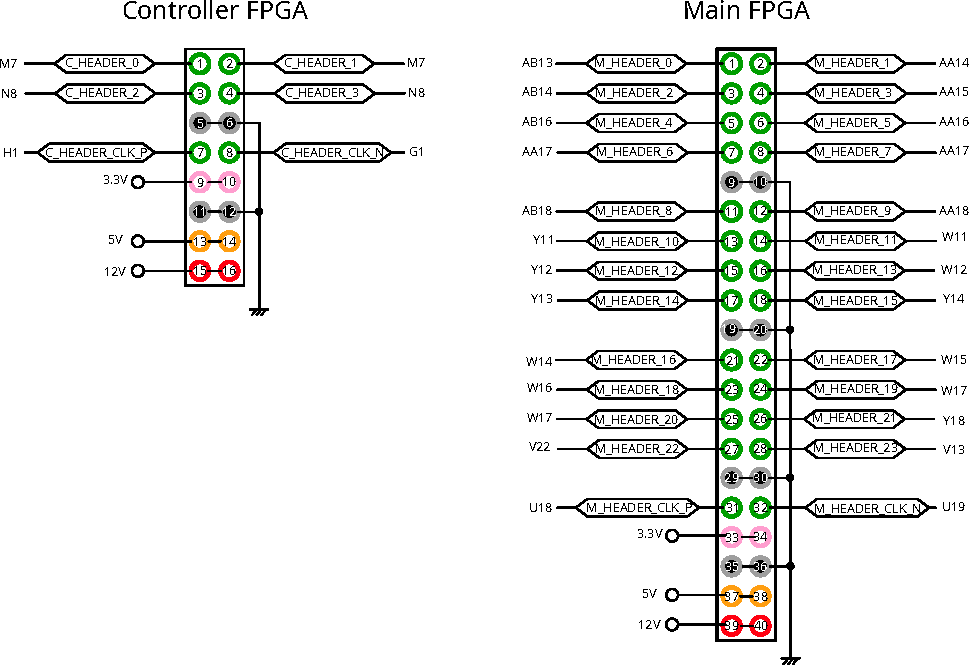
\includegraphics[width=120mm]{images/Pinheader.pdf}
  \caption{Controller FPGAおよびMain FPGAのGPIOピンヘッダ}
  \label{fig:pinmap_fpga}
\end{figure}

\subsubsection{外部通信インタフェース}
本基板はPCとの通信インタフェースとしてFT600とFT2232Hを搭載している。FT600はControl FPGAに接続されている。FT2232Hは内部的にFT232Hが2つ入った構成であるため、それぞれMainとControlに接続されている。図\ref{fig:USB}にFPGAとPCの接続インタフェースの構成を示す。
\begin{figure}[htbp]
  \centering
  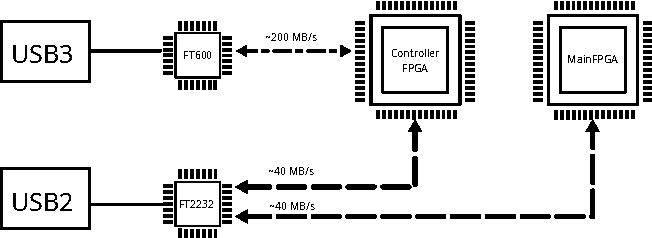
\includegraphics[width=120mm]{images/USB.pdf}
  \caption{FPGAとPCの接続インタフェース}
  \label{fig:USB}
\end{figure}

表\ref{tab:ft600}にFT600とControl FPGAとの接続ピンを示す。Control FPGAとFT600はパラレルバスで接続されている。詳細はFT600のマニュアルを確認されたい。

表\ref{tab:ft2232_control}と表\ref{tab:ft2232_main}に、それぞれControl FPGAおよびMain FPGAとFT2232Hとの接続ピンを示す。FT2232HはPCから見るとFT232Hが2台に見えるデバイスである。FT232HはUARTやSPI、FIFOのパラレルバスをサポートするデバイスであり、パラレルバスでは最大40\,MB/sの転送速度を実現する。

\begin{table}[h]
  \centering
  \caption{FT600とControl FPGAの接続}
  \label{tab:ft600}
  \small
  \renewcommand{\arraystretch}{0.9}
  \begin{tabular}{|l|l|l|} \hline
    信号名 & FT600 & Control FPGA \\ \hline \hline
    FT600\_DATA0 & DATA\_0 & H1 \\
    FT600\_DATA1 & DATA\_1 & G1 \\
    FT600\_DATA2 & DATA\_2 & F2 \\
    FT600\_DATA3 & DATA\_3 & F1 \\
    FT600\_DATA4 & DATA\_4 & E2 \\
    FT600\_DATA5 & DATA\_5 & E1 \\
    FT600\_DATA6 & DATA\_6 & D2 \\
    FT600\_DATA7 & DATA\_7 & D1 \\
    FT600\_DATA8 & DATA\_8 & C1 \\
    FT600\_DATA9 & DATA\_9 & B1 \\
    FT600\_DATA10 & DATA\_10 & B2 \\
    FT600\_DATA11 & DATA\_11 & A2 \\
    FT600\_DATA12 & DATA\_12 & B3 \\
    FT600\_DATA13 & DATA\_13 & A3 \\
    FT600\_DATA14 & DATA\_14 & B4 \\
    FT600\_DATA15 & DATA\_15 & A4 \\
    FT600\_CLK & CLK & C4 \\
    FT600\_BE0 & BE0 & H2 \\
    FT600\_BE1 & BE1 & H3 \\
    FT600\_TXE & TXE & H4 \\
    FT600\_RXF & RXF & L10 \\
    FT600\_SIWU & SIWU & G4 \\
    FT600\_WR & WR & N4 \\
    FT600\_RD & RD & E3 \\
    FT600\_OE & OE & D3 \\
    FT600\_WAKEUP & $\sim$WAKEUP & D4 \\
    FT600\_GPIO0 & GPIO0 & B5 \\
    FT600\_GPIO1 & GPIO1 & C5 \\ \hline
  \end{tabular}
\end{table}

\clearpage
\begin{table}[htbp]
  \centering
  \small
  \begin{minipage}[t]{0.48\textwidth}
    \centering
    \caption{FT2232HとControl FPGAの接続}
    \label{tab:ft2232_control}
    \begin{tabular}{|l|l|l|} \hline
      信号名 & FT2232 & Control FPGA \\ \hline \hline
      BDBUS\_D7 & BDBUS0 & N1 \\
      BDBUS\_D8 & BDBUS1 & M1 \\
      BDBUS\_D9 & BDBUS2 & M2 \\
      BDBUS\_D10 & BDBUS3 & L1 \\
      BDBUS\_D11 & BDBUS4 & K1 \\
      BDBUS\_D12 & BDBUS5 & K2 \\
      BDBUS\_D13 & BDBUS6 & J1 \\
      BDBUS\_D14 & BDBUS7 & J2 \\
      BCBUS0\_RXF\_B & BCBUS0 & P2 \\
      BCBUS1\_TXF\_B & BCBUS1 & P3 \\
      BCBUS2\_RD\_B & BCBUS2 & N2 \\
      BCBUS3\_WR\_B & BCBUS3 & N3 \\
      BCBUS4\_SIWUA & BCBUS4 & M4 \\
      BCBUS5\_CLKOUT & BCBUS5 & M3 \\
      BCBUS6\_OE\_B & BCBUS6 & K3 \\
      BCBUS7 & BCBUS7 & J3 \\
      SUSPEND\_B & SUSPEND\# & P1 \\
      PWREN\_B & PWREN\# & J4 \\ \hline
    \end{tabular}
  \end{minipage}\hfill
  \begin{minipage}[t]{0.48\textwidth}
    \centering
    \caption{FT2232HとMain FPGAの接続}
    \label{tab:ft2232_main}
    \begin{tabular}{|l|l|l|} \hline
      信号名 & FT2232 & Main FPGA \\ \hline \hline
      ADBUS\_D0 & ADBUS0 & AA10 \\
      ADBUS\_D1 & ADBUS1 & AB10 \\
      ADBUS\_D2 & ADBUS2 & AA9 \\
      ADBUS\_D3 & ADBUS3 & AB9 \\
      ADBUS\_D4 & ADBUS4 & AA8 \\
      ADBUS\_D5 & ADBUS5 & AB7 \\
      ADBUS\_D6 & ADBUS6 & AA7 \\
      ADBUS\_D7 & ADBUS7 & AB6 \\
      ACBUS0\_RXF\_B & ACBUS0 & AA6 \\
      ACBUS1\_TXF\_B & ACBUS1 & AB5 \\
      ACBUS2\_RD\_B & ACBUS2 & AB4 \\
      ACBUS3\_WR\_B & ACBUS3 & AA3 \\
      ACBUS4\_SIWUA & ACBUS4 & AB3 \\
      ACBUS5\_CLKOUT & ACBUS5 & AB2 \\
      ACBUS6\_OE\_B & ACBUS6 & AA2 \\
      ACBUS7 & ACBUS7 & AA1 \\ \hline
    \end{tabular}
  \end{minipage}
\end{table}


%==============================================================
\subsection{電力測定回路}
\label{sec:power_measure}
%==============================================================
図\ref{fig:PowerMeasure}に電力測定回路の概略図を示す。

SHAMIKOのMain FPGAコア電圧の電源ラインにはシャント抵抗が挿入されており、その両端にはBNC端子が接続されている。FPGAのコアが電力を消費するとシャント抵抗両端の電位差が変化するため、演算により消費される電力が電位差となって現れる。

SHAMIKOに搭載されているFPGAはSpartan-7であり、Spartan-7にはコア電圧であるVCC\_INTとBRAMの電源であるVCC\_BRAMが存在する。SHAMIKOでは、コア電源のみ、もしくはコア電源およびBRAM電源の両方の消費電力を測定可能になっている。この切り替えは、基板上にある0\,$\Omega$のジャンパー抵抗で行う。また、SHAMIKOのコア電源は電圧変化を平滑化させないために、バイパスコンデンサをデフォルトで未実装としている。一方、BRAM電源にはデフォルトでバイパスコンデンサが接続されているため、必要に応じて除去されたい。

SHAMIKOの消費電力の測定方法は二種類存在する。
\begin{enumerate}
  \item \textbf{基板上のアンプによる測定}：SHAMIKOの基板上にはSAKURA-Gと同等の電圧増幅回路が設置されている。この増幅回路の出力はBNC端子に接続されているため、オシロスコープに接続するだけで電力を観察することができる。
  \item \textbf{シャント抵抗両端の直接測定}：シャント抵抗の両端にはBNC端子が存在する。この2つのBNC端子を差動増幅回路に入力し、電位差の変化を観察することでも消費電力変動を観測することが可能である。
\end{enumerate}

\begin{figure}[htbp]
  \centering
  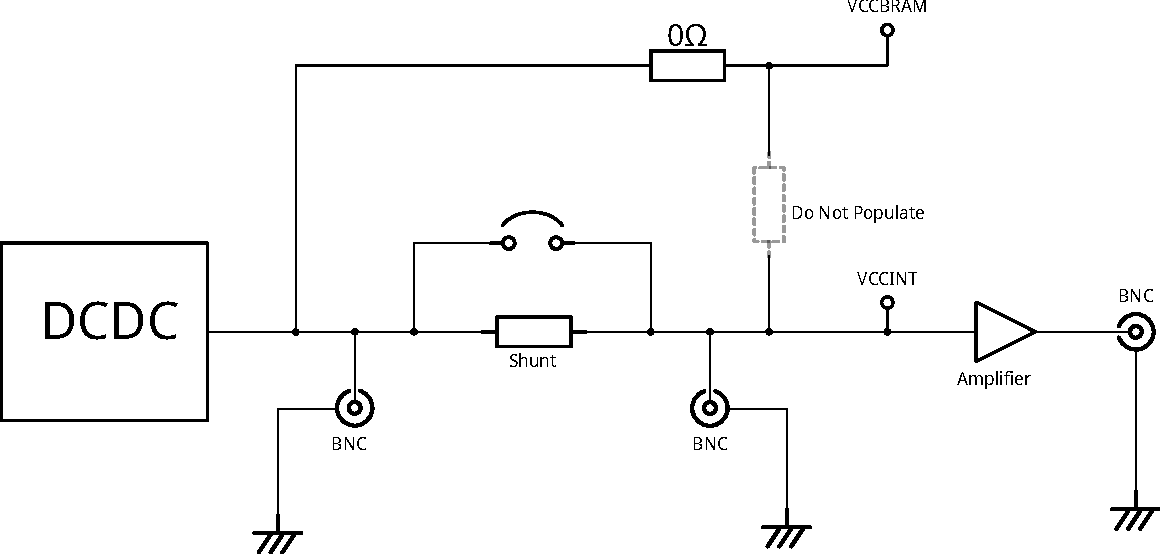
\includegraphics[width=100mm]{images/PowerMeasure.pdf}
  \caption{電力測定回路の概略図}
  \label{fig:PowerMeasure}
\end{figure}

%==============================================================
\section{基板設計データ}
%==============================================================
以下回路図を連結
\end{document}